\documentclass[a4paper]{article}
%\usepackage{spconf,amsmath,amssymb,graphicx}
\usepackage{amsmath,amssymb,graphicx,caption,listings,hyperref,graphicx,verbatim, geometry}

% Example definitions.
% --------------------
% nice symbols for real and complex numbers
\newcommand{\R}[0]{\mathbb{R}}
\newcommand{\C}[0]{\mathbb{C}}
% bold paragraph titles
\newcommand{\mypar}[1]{{\bf #1.}}
\newcommand{\mysubpar}[2]{{\bf #1.}}
\graphicspath{ {./images/} }
\geometry{a4paper, top=2cm, bottom=2cm, left=2.5cm, right=2.5cm, heightrounded, bindingoffset=5mm}

\lstset{frame=tb,
  language=C,
  aboveskip=5mm,
  belowskip=5mm,
  showstringspaces=true,
  columns=flexible,
  numbers=none,	
  breaklines=true,
  breakatwhitespace=true,
  tabsize=2
}

\begin{document}

\title{The Reinforcement Learning for Structural Evolution method on a Docker Environment}


\author{\IEEEauthorblockN{Ivan Buccella and Matteo Maiorano}
\IEEEauthorblockA{\\Department of Computer Science\\
 University of Salerno\\
 Italy}
}
\date{} % clear date

\maketitle

\section*{Abstract}
The ReLeaSE (Reinforcement Learning for Structural Evolution) method is a new computational strategy for de novo design of molecules with desired properties.
In this document we present an execution of a novel method to generate de novo chemical compounds with desired physical, chemical and/or bioactive properties based on Deep Reinforcement Learning. The execution of the method uses a simple representation of molecules only through SMILES (simplified molecular-input line-entry system) strings and is able to predict different properties like logP, Tm, and pIC50; thanks to that, the model can learn to select the most promising molecules for further study or new drug development. 
The model integrates two deep neural networks, one generative and one predictive, which are trained separately but used jointly to generate new targeted chemical libraries. The generative models are trained with a stack-augmented memory network to produce chemically feasible SMILES strings, and predictive models are derived to predict the desired properties of the generated de novo compounds. In the first stage of the method, the generative and predictive models are trained separately with a supervised learning algorithm. In the second stage, both models are jointly trained with the Reinforcement Learning approach to guide the generation of new chemical structures toward those with the desired physical and/or biological properties.
Based on these explanations, the main work focuses on the execution of the method by training a recurrent neural network to predict logP from SMILES; in addition, several optimizations to the code are applied in order to create a platform-independent executable code using modern technologies like Docker and Docker Compose.

\section{Introduction}\label{sec:intro}

The World Economic Forum has called the combination of big data and artificial intelligence (AI) the fourth industrial revolution, capable of radically transforming science. AI is revolutionizing several fields of medicine, such as radiology, pathology and other specialties, and has begun to be used in drug discovery through deep reinforcement learning (DRL) technologies. 
Deep reinforcement learning (DRL) combines the capabilities of deep learning and reinforcement learning (RL). In RL, an agent learns to interact with its environment in order to maximize a reward. He does this through trial and error, receiving positive rewards for actions that bring him closer to his goal and negative rewards for actions that take him further away. DRL involves using deep neural networks as function approximators to learn the value function or policy in a RL problem. The value function tells the agent how good a particular state is, while the policy tells the agent what actions to take in a specific state. Although there are many synthetically feasible chemicals that could be considered as possible drug-like molecules, their huge number makes it impossible to systematically examine all of them and verify them through the construction and evaluation of each individual compound. Deep neural networks are particularly suited to this task as they can process high-dimensional data and can learn complex relationships between states and actions. These technologies are being applied in different areas, such as molecular docking, transcriptomics, understanding reaction mechanisms, and molecular energy prediction.
In drug discovery, a crucial step is to formulate a well-reasoned hypothesis on how to synthesize new compounds or select them from available chemical libraries based on structure-activity relationship (SAR) data. Automated design approaches to create compounds with specific properties have been the subject of research for the past 15 years. 
Tm (melting point) is the temperature at which a solid changes to a liquid state. In chemistry and medicinal chemistry, the melting point of a substance is often used as an identifying property because each substance has a specific melting point. Melting point is an important chemical property because it can affect a compound's stability and shelf life, as well as its safety and bioavailability.
Inhibitory concentration (IC) is a measure of the effectiveness of a chemical compound in inhibiting the activity of a particular biological target, such as an enzyme or protein. The pIC50 is a measure of the biological activity of a chemical compound, and is often used to evaluate the efficacy of a drug or other biological compound. The pIC50 is calculated as the negative logarithm of the concentration of a compound that is required to achieve a specific biological effect. The higher the pIC50 of a compound, the higher its biological activity.
The partition coefficient (P) measures how much of a solute dissolves in the water portion relative to the organic portion. It is often used to predict the distribution of a compound within the human body, as LogP can help determine whether a compound will be more soluble in fat or water.In the field of machine learning, the partition coefficient (logP) can be used as a property of a chemical compound to predict its toxicity or biological activity.
In this document we present an execution of a novel method to generate de novo chemical compounds with desired physical, chemical and/or bioactive properties based on DRL. The execution of the method, called ReLeaSE (Reinforcement Learning for Structural Evolution), uses a simple representation of molecules only through SMILES (simplified molecular-input line-entry system) strings and is able to predict different properties like logP, Tm, and pIC50; thanks to that, the model can learn to select the most promising molecules for further study or new drug development. 
The simplified molecular-input line-entry system (SMILES) is a specification in the form of a line notation for describing the structure of chemical species using short ASCII strings. SMILES strings can be imported by most molecule editors for conversion back into two-dimensional drawings or three-dimensional models of the molecules.
For example, the model could be trained to select molecules with a high logP because they have a higher probability of being biologically active. Conversely, the model could be trained to exclude molecules with too high a logP because they might be too toxic.
In the following sections we will look in detail at the use of ReLeaSe.

\mypar{Related work} 
In the "Generating focused molecule libraries for drug discovery with recurrent neural networks." \cite{generating-focused-molecule} work, it is shown that recurrent neural networks can be trained as generative models for molecular structures, similar to statistical language models in natural language processing. The work has demonstrated that the properties of the generated molecules correlate very well with the properties of the molecules used to train the model. In order to enrich libraries with molecules active toward a given biological target, it has been proposed to fine-tune the model with small sets of molecules, which are known to be active against that target. Against Staphylococcus aureus, the model reproduced 14\% of 6051 hold-out test molecules that medicinal chemists designed, whereas, against Plasmodium falciparum (Malaria), it reproduced 28\% of 1240 test molecules. When coupled with a scoring function, the model can perform the complete de novo drug design cycle to generate large sets of novel molecules for drug discovery. 
In the "Molecular de novo design through deep reinforcement learning" \cite{molecular-denovo-design} has beeen introduce a method to tune a sequence-based generative model for molecular de novo design that through augmented episodic likelihood can learn to generate structures with certain specified desirable properties. The work has demonstrated how this model can execute a range of tasks such as generating analogues to a query structure and generating compounds predicted to be active against a biological target. As proof of principle, the model is first trained to generate molecules that do not contain sulphur. As a second example, the model is trained to generate analogues to the drug Celecoxib, a technique that could be used for scaffold hopping or library expansion starting from a single molecule. Finally, when tuning the model towards generating compounds predicted to be active against the dopamine receptor type 2, the model generates structures of which more than 95\% are predicted to be active, including experimentally confirmed actives that have not been included in either the generative model or the activity prediction model.

\textit{The generative
model in references (23, 37) is a “vanilla” RNN without augmented
memory stack, which does not have the capacity to count and infer
algorithmic patterns (34).
}

\section{The Method}\label{sec:The Method}

The ReLeaSE method implements a DRL approach for de novo design of novel chemical compounds with desired properties. ReLeaSE is distinguished from other similar approaches by its simple representation of molecules through the molecular string input system (SMILES) only during the generation and prediction phases of the method and the integration of these phases into a single workflow that also includes an RL module. 
The project makes use of QSPR (Quantitative Structure-Property Relationship) a technique that uses mathematical models to predict the properties of a chemical compound based on its chemical structure. QSPR models are based on the assumption that there is a quantitative relationship between the structure of a chemical compound and its properties. To build a QSPR model, data on the structure and properties of a large number of known chemical compounds (training set) are used, which are then used to train the model. Once the model has been trained, it can be used to predict the properties of unknown chemical compounds (test set). QSPR models are very useful because they make it possible to predict the properties of a chemical compound without having to synthesize or test it experimentally.
The training process consists of two stages: in the first stage the generative model is built.
Since Regular Recurring Neural Networks (RNNs) such as long short-term memory (LSTM) \cite{lstm} and gated recurrent unit (GRU) \cite{gru} are unable to solve the sequence prediction problems because of their inability to count, for the generative model, a special type of stack-augmented RNN (Stack-RNN) \cite{stack-rnn} has been used; that has found success in inferring algorithmic patterns. This Stack-RNN defines a new neuron or cell structure on top of the standard gated recurrent unit \cite{grnn} cell (see Fig. \ref{fig:softmax-loss} - A). It has two additional multiplicative gates referred to as the memory stack, which allow the Stack-RNN to learn meaningful long-range interdependencies. Stack memory is a differentiable structure onto and from which continuous vectors are inserted and removed. The objective of the Stack-RNN then is to learn hidden rules of forming sequences of letters that correspond to legitimate SMILES strings.
The generative model has two modes of processing sequences—training and generating.  
At each time step, during the training mode, the generative network takes a current prefix of the training object and predicts the probability distribution of the next character (Fig. \ref{fig:softmax-loss}). 

\begin{figure}[htbp]
    \centering
        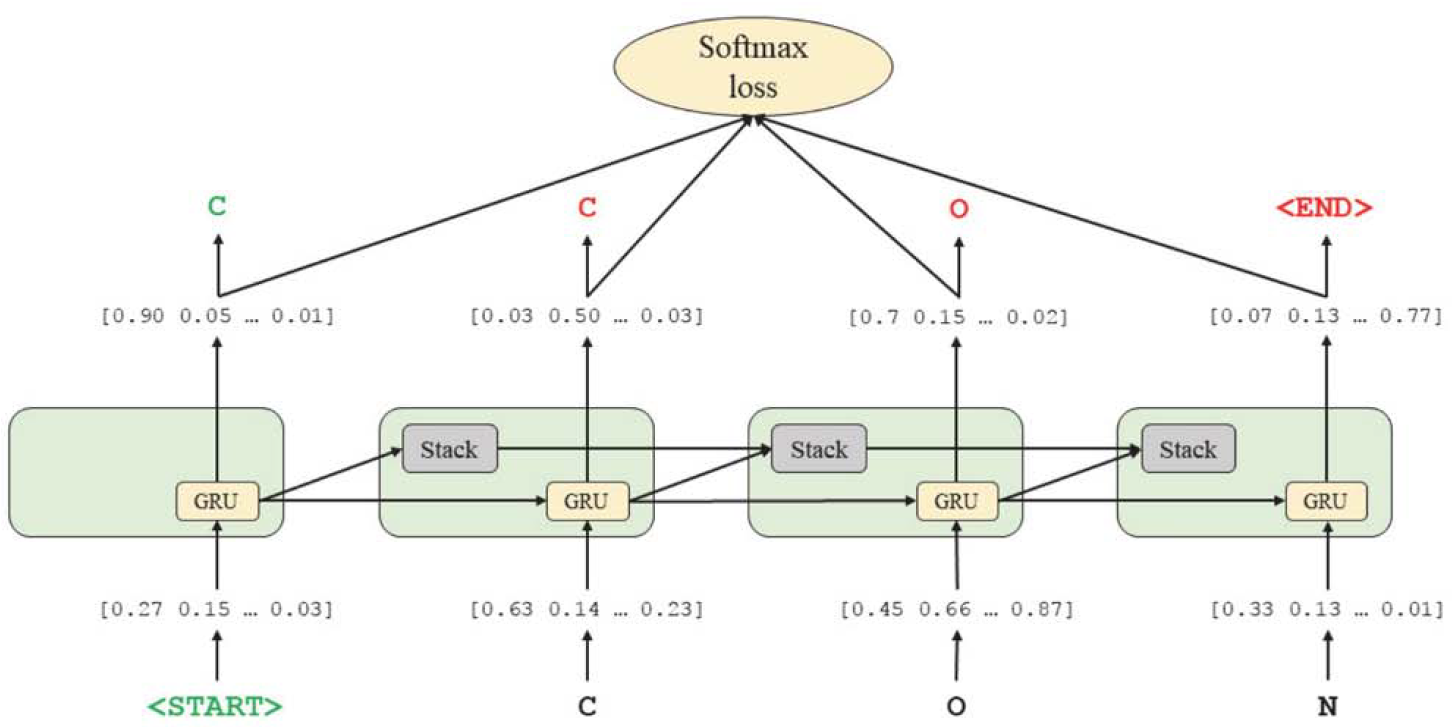
\includegraphics[width=\textwidth]{softmax-loss.png}
    \caption{Training step of the generative Stack-RNN}
    \label{fig:softmax-loss}
\end{figure}
	
Then, the next character is sampled from this predicted probability distribution and is compared to the ground truth. Afterward, on the basis of this comparison, the cross-entropy loss function is calculated, and parameters of the model are updated. 
At each time step, in generating mode, the generative network takes a prefix of already generated sequences and then, like in the training mode, predicts the probability distribution of the next character and samples it from this predicted distribution (Fig. \ref{fig:predicted-distribution}). 

\begin{figure}[htbp]
    \centering
        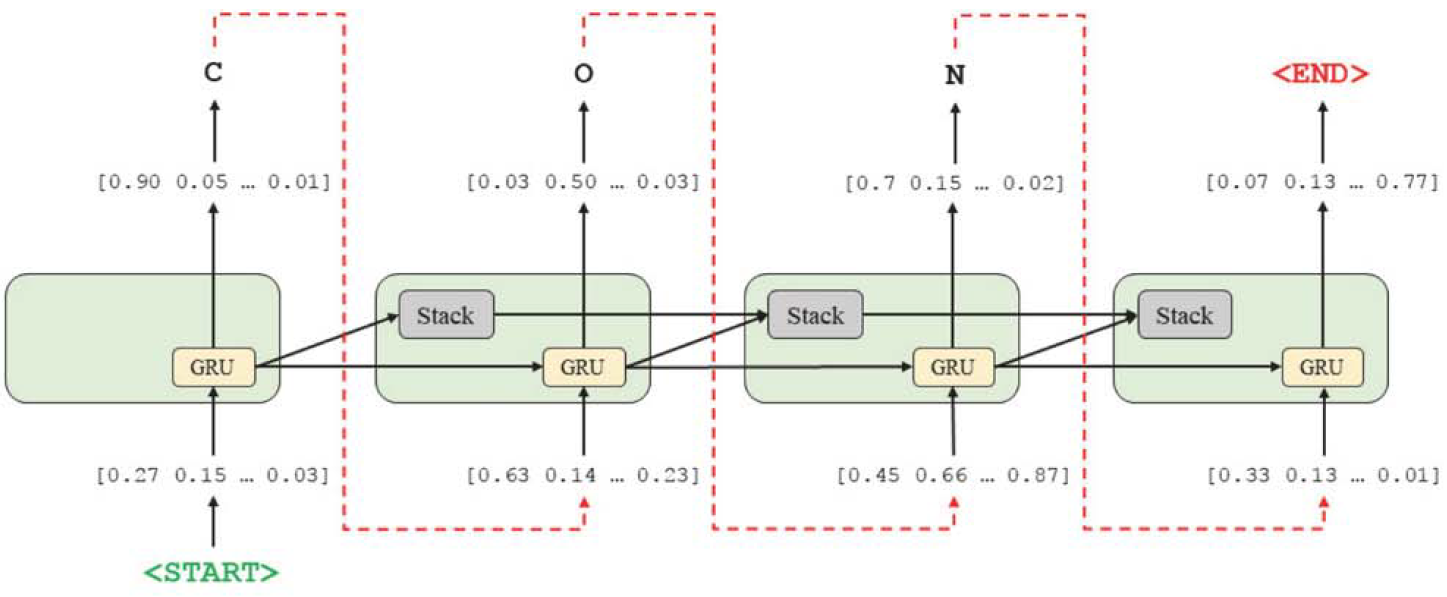
\includegraphics[width=\textwidth]{predicted-distribution.png}
    \caption{Generator step of the generative Stack-RNN}
    \label{fig:predicted-distribution}
\end{figure}
	
In the generative model, the model parameters are not updated. 
At the second stage, both generative and predictive models are combined into one Reinforcement Learning system, as shown in figure \ref{fig:parameter-optimization}. 

\begin{figure}[htbp]
    \centering
        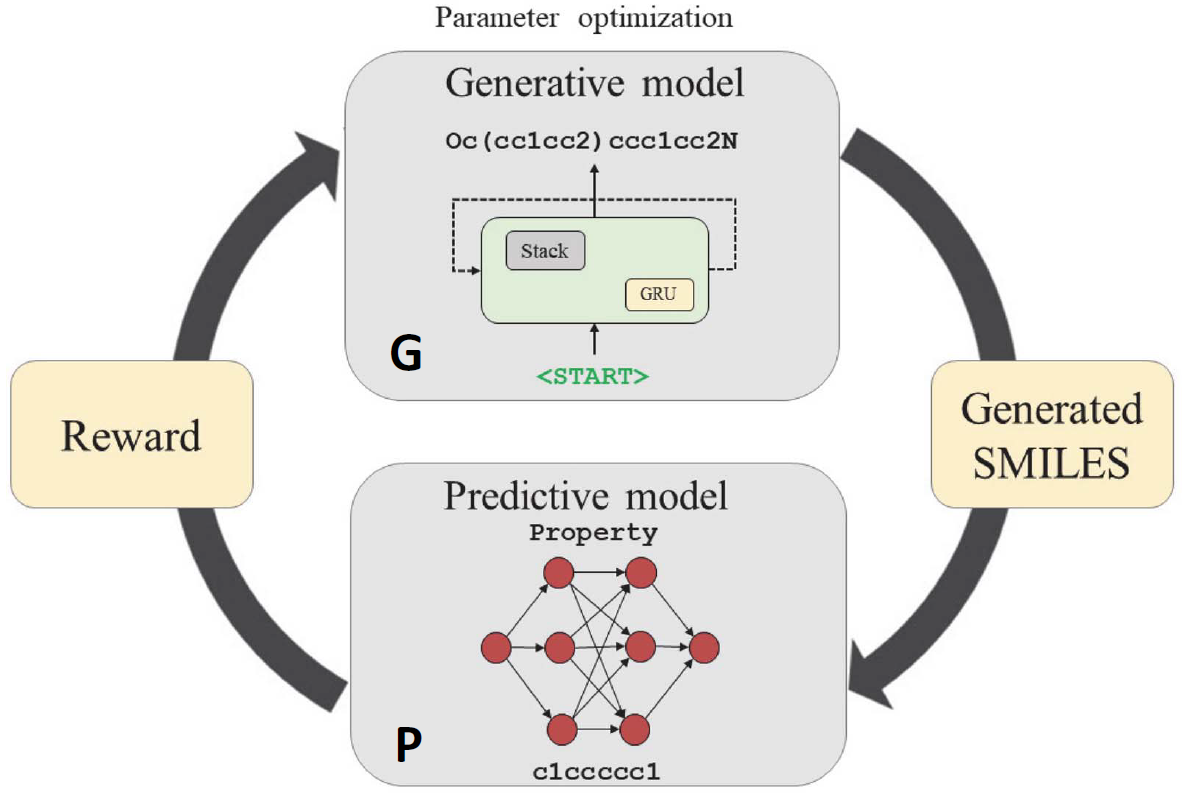
\includegraphics[width=\textwidth]{parameter-optimization.png}
    \caption{General pipeline of RL system for novel compound generation}
    \label{fig:parameter-optimization}
\end{figure}

In this system, the generative model G (Fig. \ref{fig:parameter-optimization}) plays the role of an agent, whose action space is represented by the SMILES notation alphabet, and state space is represented by all possible strings in this alphabet. The predictive model plays the role of a critic estimating the agent's behavior by assigning a numerical reward to every generated molecule. 
The predictive model P (Fig. \ref{fig:parameter-optimization}) is a model for estimating physical, chemical, or biological properties of molecules. This property prediction model is a deep neural network, which consists of an embedding layer, an LSTM layer, and two dense layers. This network is designed to calculate user-specified property (activity) of the molecule taking a SMILES string as an input data vector. This model takes a SMILES string as an input and provides one real number, which is an estimated property value, as an output (Fig. \ref{fig:smiles-to-predicted-property}). In a practical sense, this learning step is analogous to traditional  quantitative structure-activity relationships (QSAR) models. However, unlike conventional QSAR, no numerical descriptors are needed, as the model distinctly learns directly from the SMILES notation as to how to relate the comparison between SMILES strings to that between target properties. The predictor uses, as shown in the figure \ref{fig:smiles-to-predicted-property}, two unidirectional LSTM layers with hidden size of 128 each, with an embedding size of 128. The dense layer is a Multi-layer Perceptron with hidden size of 128 and ReLU activation function.

\begin{figure}[htbp]
    \centering
        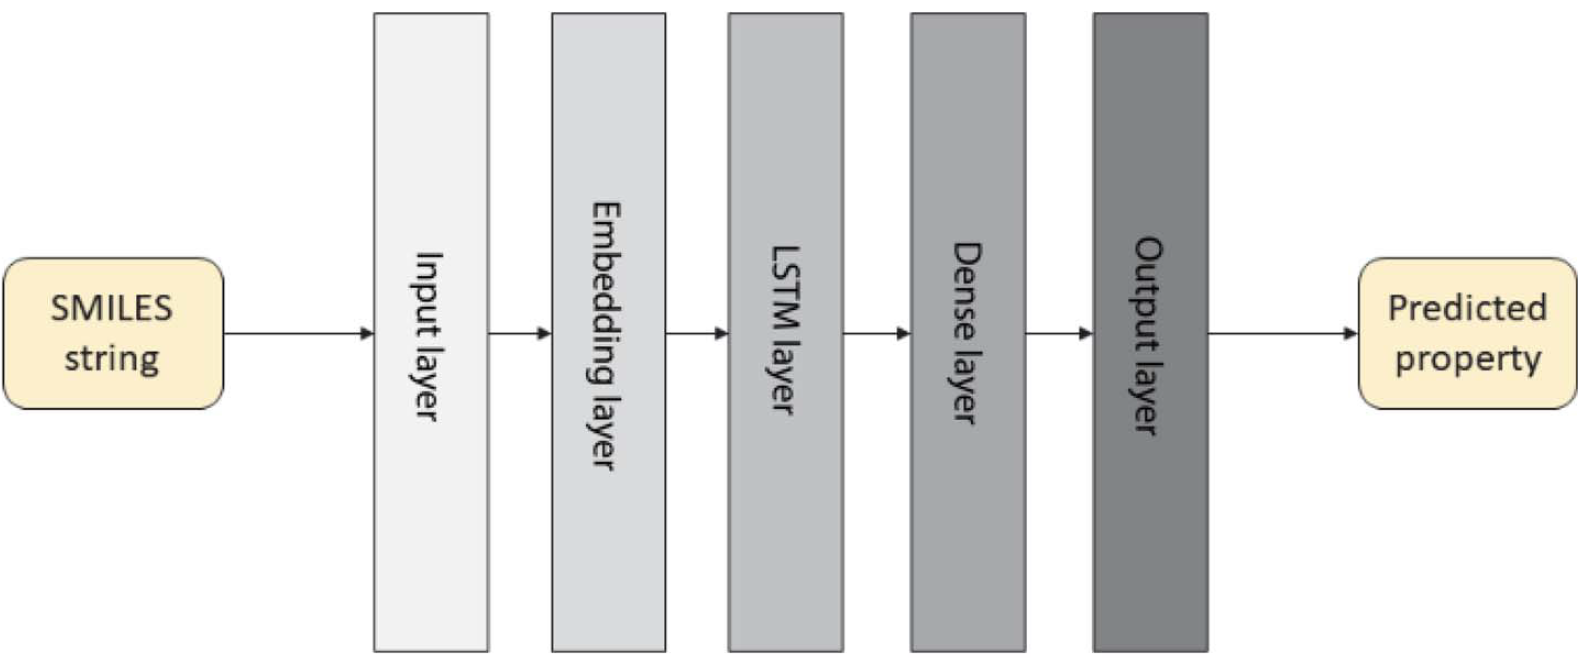
\includegraphics[width=\textwidth]{smiles-to-predicted-property.png}
    \caption{Scheme of predictive model.}
    \label{fig:smiles-to-predicted-property}
\end{figure}
	
The reward (Fig. \ref{fig:parameter-optimization}) is a function of the numerical property calculated by the predictive model. At this stage, the generative model is trained to maximize the expected reward.
The absolute majority of compounds generated de novo by the ReLeaSE method are novel structures as compared to the data sets used to train generative models, and any traditional quantitative structure-activity relationships model could be used to evaluate their properties.
As a proof of principle, the method has been tested on three diverse types of endpoints: physical properties, biological activity, and chemical substructure bias. The use of a flexible reward function enables different library optimization strategies where one can minimize,maximize, or impose a desired range to a property of interest in the generated compound libraries.

\section{The execution}\label{sec:The execution}

In this experiment we will optimize parameters of pretrained generative RNN to produce molecules with values of logP within drug-like regions according to Lipinsky rule. We use policy gradient algorithm with custom reward function to bias the properties of generated molecules.
The following example uses real SMILES strings, contained in a given input file (we used the ChEMBL database of drug-like compounds).
In this execution the generator produces a new SMILES string, which is then evaluated by the predictor. Based on the obtained prediction and the goal, it is assigned a numerical reward value and updated the parameters of the generator using policy gradient algorithm.
 
The policy gradient loss is defined as follow:

\begin{figure}[htbp]
    \centering
        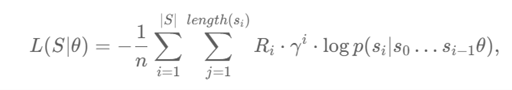
\includegraphics[width=0.70\textwidth]{formula.png}
    \label{fig:formula}
\end{figure}

where \textit{R} is the reward obtained at time step i. \begin{math}\gamma\end{math} is the discount factor and \begin{math} p(s_i | s_1,\cdots ,s_i_-_1,\theta) \end{math} is the probability of the next character given the prefix, which is obtained from the generator. The reward is the same for every time step and is equal to the reward for the whole molecule. 

\subsection{Prerequisites}\label{sec:Prerequisites}

\begin{itemize}
	\item Linux OS or WSL 2 on a Windows 10 (or higher) machine. If you use WSL 2, follow the \href{https://docs.nvidia.com/cuda/wsl-user-guide/index.html#getting-started-with-cuda-on-wsl}{[official guide]}.
	\item A Modern NVIDIA GPU, compatible with \href{https://developer.nvidia.com/cuda-11.3.0-download-archive}{[CUDA 11.3]}.
	\item Docker and Docker Compose (Application containers engine). Install it from \href{https://www.docker.com}{[here]}.
	\item The Docker GPU Support enabled on the machine; check it out \href{https://docs.docker.com/compose/gpu-support/}{[here]}.
	\item The Nvidia Container Toolkit. Install it from \href{https://docs.nvidia.com/datacenter/cloud-native/container-toolkit/install-guide.html#install-guide}{[here]}.
\end{itemize}

\begin{flushleft}
Note that you do not need to install the CUDA Toolkit on the host system.

Note that you have to install the NVIDIA drivers on your system.
\end{flushleft}


\section{Installation}\label{sec:Installation}

In this section is described how to implement and run the ReLeaSe method on a machine.

\subsection{Instructions}\label{sec:Instructions}

As mentioned into the \href{https://github.com/IvanBuccella/SF2Bio#installation}{repository} of the project, the following instructions need to be performed for running the container:

\begin{lstlisting}
1 git clone https://github.com/IvanBuccella/SF2Bio
2 cd docker
3 Set your own environment variables (the jupyter notebook port) by using the '.env-sample' file. You can just duplicate and rename it in '.env'.
4 docker-compose build
5 docker-compose up
\end{lstlisting}

\subsection{The Dockerfile}\label{sec:The Dockerfile}

During the installation and initialization phases of the project, some changes had to be made to the code to resolve errors that prevented it from starting. This could have been caused by several factors, such as the presence of outdated dependencies or incompatible package versions. These changes allowed the use of newer versions of the packages, which were more stable and compatible with the code. 
The result of this phase gave in output the construction of the Dockerfile which replicates the installation methodology described in the ReLeaSe method \href{https://github.com/isayev/ReLeaSE#installation-with-anaconda}{repository}. 

\begin{lstlisting}[label={lst:dockerfile}]
1 FROM nvidia/cuda:11.3.0-cudnn8-runtime-ubuntu20.04
2 RUN apt-get update
3 RUN apt-get install -y git
4 RUN apt-get install -y wget
5 RUN wget https://repo.anaconda.com/miniconda/ Miniconda3-latest-Linux-x86_64.sh
6 RUN bash Miniconda3-latest-Linux-x86_64.sh -b -p /miniconda
7 ENV PATH=\$PATH:/miniconda/pcondabin:/miniconda/bin
8 RUN conda update -n base -c defaults conda
9 RUN conda create -n release python=3.6
10 SHELL ["conda","run","-n","release","/bin/bash", "-c"]
11 COPY environment environment
12 RUN conda install --yes --file environment/conda.txt
13 RUN conda install -c rdkit rdkit nox cairo
14 RUN conda install pytorch=1.10.1 torchvision=0.11.2 -c pytorch -c conda-forge
15 RUN pip install -r environment/pip.txt
16 WORKDIR /home
17 RUN git clone https://github.com/isayev/ReLeaSE.git .
18 ENTRYPOINT ["conda", "run", "-n", "release", "jupyter", "notebook", "--ip=0.0.0.0", "--port=8888", "--allow-root", "--NotebookApp.token=''", "--NotebookApp.password=''"]
\end{lstlisting}

As shown in the code above, build starts from the official \href{https://hub.docker.com/r/nvidia/cuda}{Nvidia CUDA docker image} with Ubuntu 20.04. To the initial image, several dependencies are added, like \href{https://docs.conda.io/en/latest/miniconda.html}{MiniConda} which is a bootstrap version of Anaconda [Row 5 of \ref{lst:dockerfile}].
Once Conda is installed, a new environment with Python is created [Row 11 of \ref{lst:dockerfile}] and the required dependencies specified in the conda.txt file are installed [Row 12 of \ref{lst:dockerfile}]. In addition, RDKit, Nox, Cairo, pytorch and torchvision are installed [Rows 13-14 of \ref{lst:dockerfile}]. 
Then the pip dependencies listed in the pip.txt file, such as \href{https://www.tensorflow.org/tensorboard}{tensorboard}, \href{https://www.tensorflow.org/}{tensorflow} are installed [Row 15 of \ref{lst:dockerfile}].
Finally, the ReLeaSe code repository is cloned into the workdir of the image and the entrypoint of the jupyter notebook is defined.

\subsection{The Docker Compose}\label{sec:The Docker Compose}

\begin{lstlisting}
1  version: "3.8"
2  services:
3   app:
4     platform: linux/amd64
5     build:
6       context: .
7       dockerfile: Dockerfile
8     environment:
9       - NVIDIA_DISABLE_REQUIRE=1
10    ports:
11     - \${HTTP_PORT}:8888
12    deploy:
13      resources:
14        reservations:
15          devices:
16            - capabilities: [gpu]
\end{lstlisting}

As shown in the code above, the docker-compose file includes the GPU access \cite{gpu-support} to the service container “app” including all the nvidia GPUs installed on the host machine. This access allows the container to use the nvidia GPUs shared for the execution; in particular this allows “pytorch” to find and to use the CUDA cores.

\subsection{The running container}\label{sec:The running container}

\begin{figure}[htbp]
    \centering
        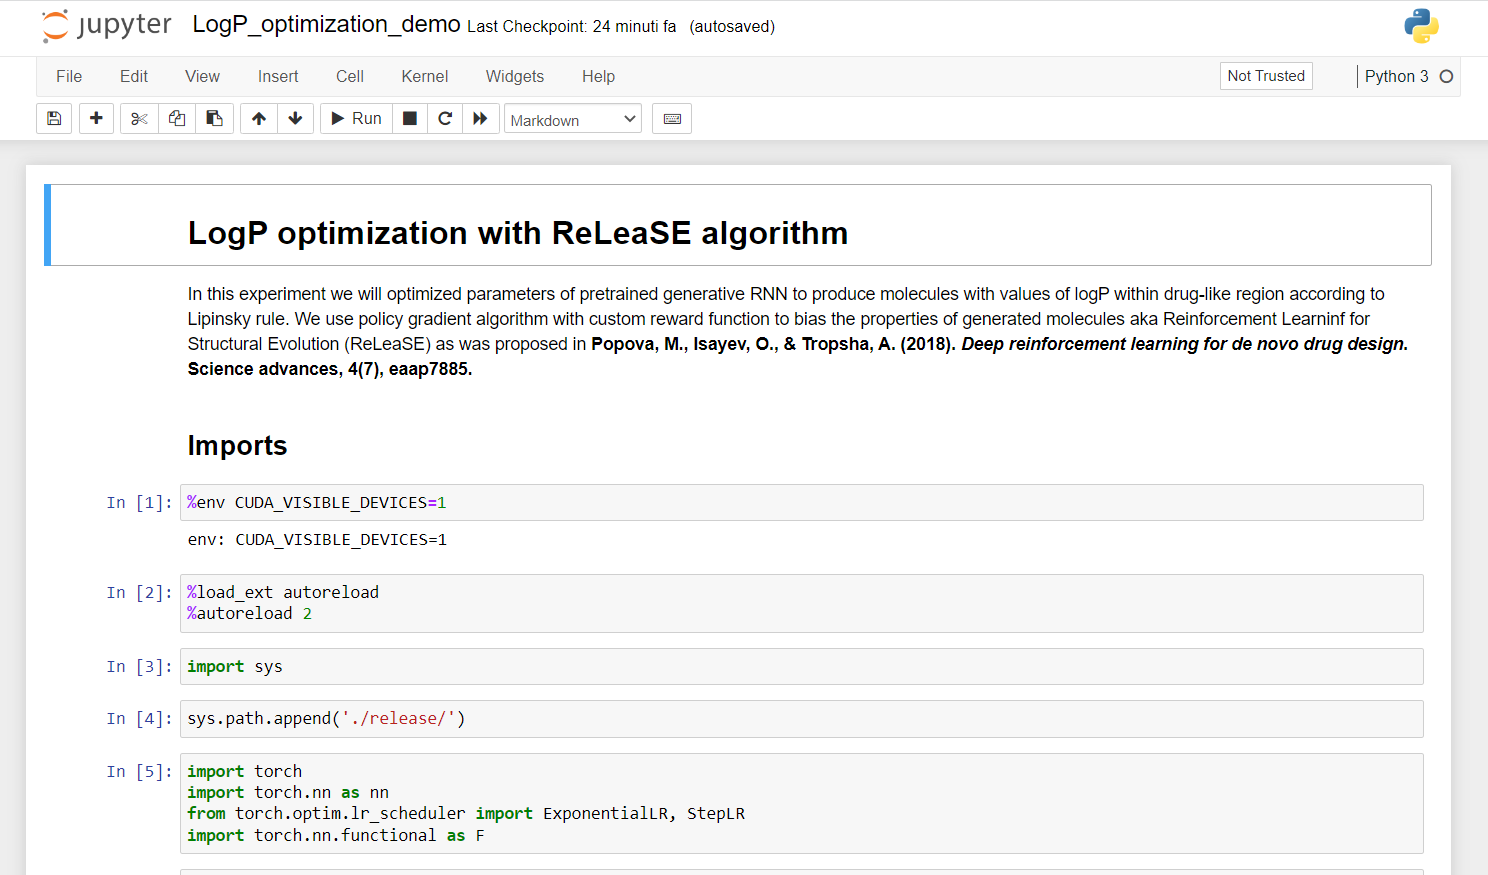
\includegraphics[width=\textwidth]{logp-optimization.png}
    \label{fig:logp-optimization}
\end{figure}

In the figure above is reported the configured jupyter notebook of the execution described in the following sections; it can be reached by visiting the \href{http://localhost:{HTTP_PORT}/LogP_optimization_demo.ipynb}{URL} into the host machine web browser.

\section{Description of the execution}\label{sec:Description of the execution}

\subsection{First stage - Setting up the generator}\label{sec:First stage - Setting up the generator}

The real SMILES strings, aka the data, are read from the ChEMBL database; they are included into a .smi file:

\begin{lstlisting}
gen_data_path = './data/chembl_22_clean_1576904_sorted_std_final.smi'
tokens = ['<', '>', '#', '%', ')', '(', '+', '-', '/', '.', '1', '0', '3', '2', '5', '4', '7',
          '6', '9', '8', '=', 'A', '@', 'C', 'B', 'F', 'I', 'H', 'O', 'N', 'P', 'S', '[', ']',
          '\\', 'c', 'e', 'i', 'l', 'o', 'n', 'p', 's', 'r', '\n']
gen_data = GeneratorData(training_data_path=gen_data_path, delimiter='\t', 
                         cols_to_read=[0], keep_header=True, tokens=tokens)
\end{lstlisting}

Then the stack-augmented generative RNN is initialized:

\begin{lstlisting}
hidden_size = 1500
stack_width = 1500
stack_depth = 200
layer_type = 'GRU'
lr = 0.001
optimizer_instance = torch.optim.Adadelta

my_generator = StackAugmentedRNN (input_size=gen_data.n_characters, hidden_size=hidden_size,
									 output_size=gen_data.n_characters, layer_type=layer_type,
									 n_layers=1, is_bidirectional=False, has_stack=True,
									 stack_width=stack_width, stack_depth=stack_depth, 
									 use_cuda=use_cuda, 
									 optimizer_instance=optimizer_instance, lr=lr)
model_path = './checkpoints/generator/checkpoint_biggest_rnn'
losses = my_generator.fit(gen_data, 1500000)
plt.plot(losses)
my_generator.evaluate(gen_data)
my_generator.save_model(model_path)
my_generator.load_model(model_path)
\end{lstlisting}

\subsection{First stage - Build the Predictive Recurrent Neural Network}\label{sec:First stage - Build the Predictive Recurrent Neural Network}

The stack-augmented predictive RNN is generated. 

The data are read from the following code:

\begin{lstlisting}
from openchem.data.utils import read_smiles_property_file
data = read_smiles_property_file('./data/logP_labels.csv', 
                                 cols_to_read=[1, 2], keep_header=False)
smiles = data[0]
labels = data[1].astype('float32')
\end{lstlisting}

The imported data are prepared:

\begin{lstlisting}
from openchem.data.utils import get_tokens
tokens, _, _ = get_tokens(smiles)
tokens = ['<', '>', '#', '%', ')', '(', '+', '-', '/', '.', '1', '0', '3', '2', '5', '4', '7',
          '6', '9', '8', '=', 'A', '@', 'C', 'B', 'F', 'I', 'H', 'O', 'N', 'P', 'S', '[', ']',
          '\\', 'c', 'e', 'i', 'l', 'o', 'n', 'p', 's', 'r', '\n']
tokens = ''.join(tokens) + ' '

from sklearn.model_selection import KFold, train_test_split

cross_validation_split = KFold(n_splits=5, shuffle=True)

data = list(cross_validation_split.split(smiles, labels))
\end{lstlisting}

The model parameters are configured as follow:

\begin{lstlisting}
import torch
from openchem.utils.utils import identity
from openchem.modules.embeddings.basic_embedding import Embedding
model_object = Smiles2Label

n_hidden = 128
batch_size = 128
num_epochs = 26
lr = 0.005

model_params = {
    'use_cuda': True,
    'random_seed': 42,
    'world_size': 1,
    'task': 'regression',
    'data_layer': SmilesDataset,
    'use_clip_grad': False,
    'batch_size': batch_size,
    'num_epochs': num_epochs,
    'logdir': './checkpoints/logP/',
    'print_every': 1,
    'save_every': 5,
    'train_data_layer': None,
    'val_data_layer': None,
    'eval_metrics': r2_score,
    'criterion': nn.MSELoss(),
    'optimizer': Adam,
    'optimizer_params': {
        'lr': lr,
    },
    'lr_scheduler': ExponentialLR,
    'lr_scheduler_params': {
        'gamma': 0.98
    },
    'embedding': Embedding,
    'embedding_params': {
        'num_embeddings': len(tokens),
        'embedding_dim': n_hidden,
        'padding_idx': tokens.index(' ')
    },
    'encoder': RNNEncoder,
    'encoder_params': {
        'input_size': n_hidden,
        'layer': "LSTM",
        'encoder_dim': n_hidden,
        'n_layers': 2,
        'dropout': 0.8,
        'is_bidirectional': False
    },
    'mlp': OpenChemMLP,
    'mlp_params': {
        'input_size': n_hidden,
        'n_layers': 2,
        'hidden_size': [n_hidden, 1],
        'activation': [F.relu, identity],
        'dropout': 0.0
    }
}
\end{lstlisting}

The training is done from the following code:

\begin{lstlisting}
import os
i = 0
models = []
results = []
for split in data:
    print('Cross validation, fold number ' + str(i) + ' in progress...')
    train, test = split
    X_train = smiles[train]
    y_train = labels[train].reshape(-1)
    X_test = smiles[test]
    y_test = labels[test].reshape(-1)
    save_smiles_property_file(tmp_data_dir + str(i) + '_train.smi', 
                              X_train, y_train.reshape(-1, 1))
    save_smiles_property_file(tmp_data_dir + str(i) + '_test.smi', 
                              X_test, y_test.reshape(-1, 1))

    train_dataset = SmilesDataset(tmp_data_dir + str(i) + '_train.smi',
                           delimiter=',', cols_to_read=[0, 1], tokens=tokens,
                                 flip=False,)
    train_dataset.target = train_dataset.target
    test_dataset = SmilesDataset(tmp_data_dir + str(i) + '_test.smi',
                       delimiter=',', cols_to_read=[0, 1], tokens=tokens,
                                flip=False)
    test_dataset.target = test_dataset.target
    model_params['train_data_layer'] = train_dataset
    model_params['val_data_layer'] = test_dataset
    model_params['logdir'] = log_dir + 'fold_' + str(i)  
    ckpt_dir = model_params['logdir'] + '/checkpoint/'
    try:
        os.stat(ckpt_dir)
    except:
        os.mkdir(model_params['logdir'])
        os.mkdir(ckpt_dir)
    train_loader = create_loader(train_dataset,
                             batch_size=model_params['batch_size'],
                             shuffle=True,
                             num_workers=4,
                             pin_memory=True,
                             sampler=None)
    val_loader = create_loader(test_dataset,
                           batch_size=model_params['batch_size'],
                           shuffle=False,
                           num_workers=1,
                           pin_memory=True)
    models.append(model_object(params=model_params).cuda())
    criterion, optimizer, lr_scheduler = build_training(models[i], model_params)
    results.append(fit(models[i], lr_scheduler, train_loader, optimizer, criterion,
        model_params, eval=True, val_loader=val_loader))
    
    i = i+1
\end{lstlisting}

The evaluation is done from the following code:

\begin{lstlisting}
import numpy as np
rmse = []
auc_score = []
for i in range(5):
    test_dataset = SmilesDataset(tmp_data_dir + str(i) + '_test.smi', delimiter=',', cols_to_read=[0, 1], tokens=tokens, flip=False)
    test_dataset.target = test_dataset.target
    val_loader = create_loader(test_dataset, batch_size= model_params['batch_size'], shuffle=False, num_workers=1, pin_memory=True)
    metrics = evaluate(models[i], val_loader, criterion)
    rmse.append(np.sqrt(metrics[0]))
    auc_score.append(metrics[1])
\end{lstlisting}

And then the evaluated data are saved in order to be used in the next steps:

\begin{lstlisting}
! mv ./checkpoints/logP/fold_0/checkpoint/epoch_25 ./checkpoints/logP/fold_0.pkl
! mv ./checkpoints/logP/fold_1/checkpoint/epoch_25 ./checkpoints/logP/fold_1.pkl
! mv ./checkpoints/logP/fold_2/checkpoint/epoch_25 ./checkpoints/logP/fold_2.pkl
! mv ./checkpoints/logP/fold_3/checkpoint/epoch_25 ./checkpoints/logP/fold_3.pkl
! mv ./checkpoints/logP/fold_4/checkpoint/epoch_25 ./checkpoints/logP/fold_4.pkl
\end{lstlisting}

\subsection{First stage - Setting up the predictor}\label{sec:First stage - Setting up the predictor}

The path of the generated data from the Predictive RNN is configured:

\begin{lstlisting}
path_to_params = './checkpoints/logP/model_parameters.pkl'
path_to_checkpoint = './checkpoints/logP/fold_'
\end{lstlisting}

The unbiased distribution of the property by using the previous generator and predictor created is produced:

\begin{lstlisting}
my_predictor = RNNPredictor(path_to_params, path_to_checkpoint, predictor_tokens)
smiles_unbiased, prediction_unbiased = estimate_and_update(my_generator, my_predictor, n_to_generate=10000)
\end{lstlisting}

This phase produces in output:

\begin{figure}[htbp]
    \centering
        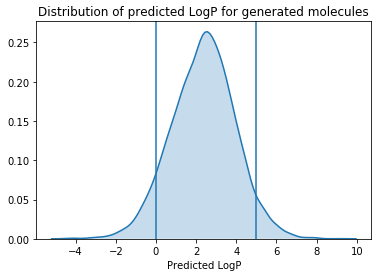
\includegraphics[width=0.70\textwidth]{unbiased.png}
    \caption{The unbiased distribution of predicted logP for generated molecules}
    \label{fig:unbiased}
\end{figure}

\subsection{Second stage - Biasing the distribution of the generator with reinforcement learning}\label{sec:Second stage - Biasing the distribution of the generator with reinforcement learning}

A copy of the generator is created:

\begin{lstlisting}
my_generator_max = StackAugmentedRNN(input_size=gen_data.n_characters, hidden_size=hidden_size, output_size=gen_data.n_characters, 
												 layer_type=layer_type,
												 n_layers=1, is_bidirectional=False, has_stack=True,
												 stack_width=stack_width, stack_depth=stack_depth, 
												 use_cuda=use_cuda, 
												 optimizer_instance=optimizer_instance, lr=lr)

my_generator_max.load_model(model_path)
\end{lstlisting}

The reward function used here is the following:

$$
R =  \begin{cases} 11.0, & \mbox{if } 1.0 < \log P < 4.0 \\ 1.0, & \mbox{otherwise}  \end{cases}
$$

\begin{lstlisting}
def get_reward_logp(smiles, predictor, invalid_reward=0.0):
    mol, prop, nan_smiles = predictor.predict([smiles])
    if len(nan_smiles) == 1:
        return invalid_reward
    if (prop[0] >= 1.0) and (prop[0] <= 4.0):
        return 11.0
    else:
        return 1.0
\end{lstlisting}

And then the Reinforcement Learning (combining the generator, the predictor and the reward function depending on the goal) is started:

\begin{lstlisting}
RL_logp = Reinforcement(my_generator_max, my_predictor, get_reward_logp)

rewards = []
rl_losses = []

for i in range(n_iterations):
	for j in trange(n_policy, desc='Policy gradient...'):
			cur_reward, cur_loss = RL_logp.policy_gradient(gen_data)
			rewards.append(simple_moving_average(rewards, cur_reward)) 
			rl_losses.append(simple_moving_average(rl_losses, cur_loss))
	
	plt.plot(rewards)
	plt.xlabel('Training iteration')
	plt.ylabel('Average reward')
	plt.show()
	plt.plot(rl_losses)
	plt.xlabel('Training iteration')
	plt.ylabel('Loss')
	plt.show()
			
	smiles_cur, prediction_cur = estimate_and_update(
																				RL_logp.generator, 
																				my_predictor, 
																				n_to_generate)
																									
	print('Sample trajectories:')
	for sm in smiles_cur[:5]:
			print(sm)
\end{lstlisting}

In this step is used an important function ''estimate\_and\_update'' which:
\begin{enumerate}
	\item generates n\_to\_generate number of SMILES strings
	\item filters invalid SMILES
	\item predicts logP for valid SMILES
	\item Returns valid SMILES and their predicted logPs
\end{enumerate}

\begin{lstlisting}
def estimate_and_update(generator, predictor, n_to_generate):
    generated = []
    pbar = tqdm(range(n_to_generate))
    for i in pbar:
        pbar.set_description("Generating molecules...")
        generated.append(generator.evaluate(gen_data, predict_len=120)[1:-1])

    sanitized = canonical_smiles(generated, sanitize=False, throw_warning=False)[:-1]
    unique_smiles = list(np.unique(sanitized))[1:]
    smiles, prediction, nan_smiles = predictor.predict(unique_smiles, use_tqdm=True)  
                                                       
    plot_hist(prediction, n_to_generate)
        
    return smiles, prediction
\end{lstlisting}

After reached the goal, the biased distribution of the property is produced:

\begin{lstlisting}
smiles_biased, prediction_biased = estimate_and_update(RL_logp.generator, my_predictor, n_to_generate=10000)
\end{lstlisting}

This phase produces in output: 

\begin{figure}[htbp]
		\centering
			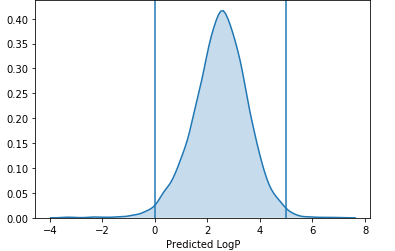
\includegraphics[width=0.70\textwidth]{biased.png}
        \caption{The biased distribution of predicted logP for generated molecules}
		\label{fig:biased}
	\end{figure}

\subsection{Output - Drawing random molecules}\label{sec:Output - Drawing random molecules}

For drawing some random compounds from the biased library, the following code can be executed:

\begin{lstlisting}
from rdkit.Chem import Draw
from rdkit.Chem.Draw import DrawingOptions
from rdkit.Chem import Draw
DrawingOptions.atomLabelFontSize = 50
DrawingOptions.dotsPerAngstrom = 100
DrawingOptions.bondLineWidth = 3
generated_mols = [Chem.MolFromSmiles(sm, sanitize=True) for sm in smiles_biased]
sanitized_gen_mols = [generated_mols[i] for i in np.where(np.array(generated_mols) != None)[0]]
n_to_draw = 20
ind = np.random.randint(0, len(sanitized_gen_mols), n_to_draw)
mols_to_draw = [sanitized_gen_mols[i] for i in ind]
legends = ['log P = ' + str(prediction_biased[i]) for i in ind]
Draw.MolsToGridImage(mols_to_draw, molsPerRow=5, 
                     subImgSize=(200,200), legends=legends)
\end{lstlisting}

The output will be something like:

\begin{figure}[htbp]
    \centering
        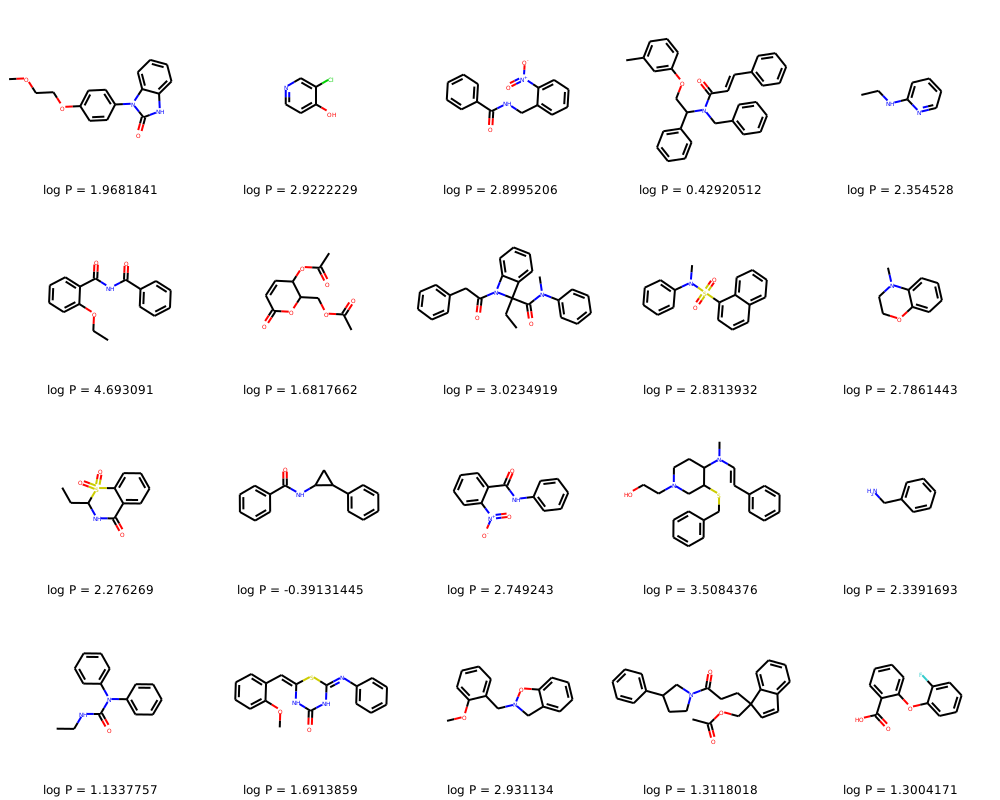
\includegraphics[width=\textwidth]{output.png}
    \label{fig:output}
\end{figure}

\begin{thebibliography}{1}

\bibitem{simplified-molecular-input-line-entry-system}
\href{https://en.wikipedia.org/wiki/Simplified_molecular-input_line-entry_system/}{Simplified molecular-input line-entry system}

\bibitem{grnn}
\href{http://arxiv.org/abs/1412.3555/}{J. Chung, C. Gulcehre, K. Cho, Y. Bengio, Empirical evaluation of gated recurrent neural networks on sequence modeling, \(2014\).}

\bibitem{stack-rnn}
\href{http://arxiv.org/abs/1503.01007}{A. Joulin, T. Mikolov, Inferring algorithmic patterns with stack-augmented recurrent nets. \(2015\)}

\bibitem{lstm}
{S. Hochreiter, J. Schmidhuber, Long short-term memory. Neural. Comput. 9, 1735-1780 \(1997\).}

\bibitem{generating-focused-molecule}
\href{https://pubs.acs.org/doi/10.1021/acscentsci.7b00512}{M. H. S. Segler, T. Kogej, C. Tyrchan, M. P. Waller, Generating focused molecule libraries for drug discovery with recurrent neural networks. ACS Cent. Sci. 4, 120-131 \(2018\).}

\bibitem{molecular-denovo-design}
\href{http://arxiv.org/abs/1704.07555}{M. Olivecrona, T. Blaschke, O. Engkvist, H. Chen, Molecular de novo design through deep reinforcement learning \(2017\).}

\bibitem{gru}
\href{http://arxiv.org/abs/1412.3555}{J. Chung, C. Gulcehre, K. Cho, Y. Bengio, Empirical evaluation of gated recurrent neural networks on sequence modeling \(2014\)}

\bibitem{gpu-support}
\href{https://docs.docker.com/compose/gpu-support/}{Docker GPU support}

\end{thebibliography}

\end{document}